%--- 41 -------------------------------%
\item\vf{L’avantage de l’utilisation de colonnes plutôt que de lignes est d’offrir un meilleur taux de
compression des données stockées.}
{\vrai}
{
En travaillant en colonnes, on peut notamment optimiser les algorithmes en fonction du types des valeurs de la colonne. (Suite réponse Q35)
}


%--- 42 -------------------------------%
\item\vf{L’avantage de l’utilisation de colonnes plutôt que de lignes est d’offrir de meilleures performances lors de la lecture de tous les enregistrements d’une table.}
{\faux}
{
Le modèle orienté-colonnes offre de meilleures performances à la lecture uniquement lorsqu'on travaille sur certaines colonnes de la table, car on utilise les fichiers relatifs à ces colonnes (et non toute la DB).
\paragraph{}
Dès lors que l'on fait une requête sur l'ensemble des enregistrements, la modèle devient un inconvénient car il nécessite d'ouvrir et de traiter TOUS les fichiers contenant les colonnes, ce qui alourdit davantage la lecture par rapport au modèle relationnel.
}


%--- 43 -------------------------------%
\item\vf{Une base HBase peut servir d’input/output de MapReduce (Hadoop)}
{\vrai}
{
HBase est un SGBD orienté-colonne qui s'exécute par dessus le système de fichiers HDFS ( = [...]). Il permet a une base de servir d'input/output de MapReduce.
\paragraph{}
Les données sont organisées dans des "\textit{tables}" identifiables par un nom. Chaque ligne possède une clé unique pour l'identifier et les colonnes sont regroupées en "\textit{familles}" (identifiables par chaines caract.). Toutes les lignes possèdent les même familles de colonnes mais celles-ci peuvent être remplies ou non.
\paragraph{}
En HBase, les données des cellules sont \textit{versionnées}. Les différentes versions sont identifiées par un \textit{Timestamp}.
\paragraph{}
Ainsi, pour obtenir la donnée d'une cellule, il faut préciser: \textit{Table --> Clé --> Famille Col. --> Colonne --> Timestamp}
\paragraph{}
Les \textbf{familles de colonnes sont stockées dans des HFile séparés}, ce qui facilite la structure de la DB et l'indexation des données. L'avantage de HBase est alors de proposer la distribution et la réplication des données sur un \textit{cluster}.
\begin{figure}[h!]
\center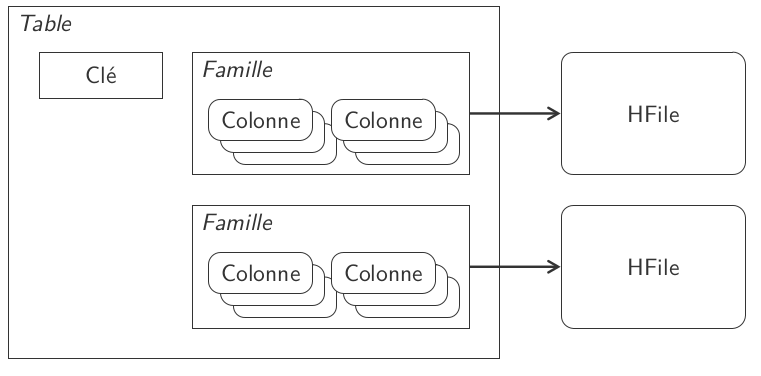
\includegraphics[scale=.3]{images/hbase}
\caption{Modèle de données en HBase \cite{ref1}}
\end{figure}

\paragraph{}
Pour l'écriture des données, celles-ci sont d'abord placées dans un buffer, le \textit{memstore}, qui écrit ensuite les changements dans un HFile [...]
\paragraph{RAPPELS MapReduce...}
}


%--- 44 -------------------------------%
\item\vf{Une base HBase peut servir de fichiers avec GFS (Google File System)}
{???}
{}


%--- 45 -------------------------------%
\item\vf{Une base de données orientée graphe stocke deux collections d’agrégats appelés nœuds et arêtes.}{\vrai}
{Le modèle orienté-graphe stocke deux types d'éléments:
\begin{itemize}
\item[$\cdot$]des \textcolor{ltred}{\textsc{noeuds}}: représentent des entités quelconques avec des propriétés
\item[$\cdot$]des \textcolor{ltred}{\textsc{arêtes}}: représentent des relations UNIDIRECTIONNELLES entre deux noeuds et possèdent une propriété. (\textit{Rem: pour faire un lien bidirictionnel, il faut donc nécessairement utiliser deux arêtes}
\end{itemize}

\paragraph{}
Puisqu'il n'y a pas de restriction sur les types des noeuds/relations, le graphe représente une collection hétérogène d'information dont l'avantage principal est de permettre une \textbf{traversée rapide} des relations, sans que celles-ci ne doivent être reconstruites.

\paragraph{}
Cette architecture est particulière utile dans les cas suivants:
\begin{itemize}
\item[$\cdot$]les collections \textit{très riche de liens} entre les entités
\item[$\cdot$]routage/dispatching et localisation
\item[$\cdot$]moteur de recommandations automatiques
\end{itemize}
}


%--- 46 -------------------------------%
\item\vf{La suppression d’un nœud dans une base de données orientée graphe implique la suppression de
toutes les relations partant et arrivant sur ce nœud.}
{\vrai}
{
Il ne peut \textbf{pas exister de lien mort} dans le graphe, autrement dit la suppression d'un noeud implique nécessairement de supprimer toutes les arêtes adjacentes.
}


%--- 47 -------------------------------%
\item\vf{Il est impossible de stocker une liste de personnes dans une base de données orientée graphe}
{\faux}
{
On distingue différents \textit{types de relations} dans le graphe dont une qui permet de représenter une \textbf{liste chaînée}. La relation est un "pointeur" vers l'élement suivant de la liste.
\begin{figure}[h!]
\center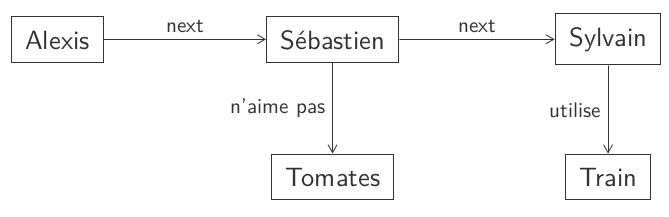
\includegraphics[scale=.3]{images/graphe-relation-liste}
\caption{Représentation d'une liste chaînée en modèle orienté-graphe \cite{ref1}}
\end{figure}
}


%--- 48 -------------------------------%
\item\vf{SPARQL est un langage de requêtes générique permettant d’interroger n’importe quelle base de
données NoSQL.}
{\faux}
{SPARQL (\textit{\textbf{S}PARQL \textbf{P}rotocol and \textbf{R}DF \textbf{Q}uery \textbf{L}anguage)} est un langage de requêtes adapté spécifiquement à la structure des graphes RDF.
\paragraph{}
Tout ceci fait partie de ce qui constitue plus communément le \textbf{Web Sémantique} qui est une extension standardisée du Web, pour l'utilisation de formats de données. Il s'agit donc du \textit{Web des données} qui permet de partager des informations structurées entre des applications. (\textit{« le Web sémantique fournit un modèle qui permet aux données d'être partagées et réutilisées entre plusieurs applications, entreprises et groupes d'utilisateurs »} W3C)
\paragraph{}
Dans ce contexte, le RDF (\textit{\textbf{R}esource \textbf{D}estcription \textbf{F}ormat}) est un \textbf{modèle de graphe} destiné à représenter de façon formelle les ressources web. Il est le langage de base du Web sémantique et permet de stocker les données sous forme de triplets "(Sujet) --- prédicat ---> (Objet)" pour marquer la relation entre deux entités.
\paragraph{}
Le SPARQL, quant à lui, est le langage de requêtes qui interroge les graphes RDF au moyen de quatre types d'instructions:
\begin{enumerate}
\item\textcolor{ltred}{\textsc{select}}: extraire un sous-graphe d'un graphe RD sous forme de table
\item\textcolor{ltred}{\textsc{construct}}: engendrer un nouveau graphe complétant un autre
\item\textcolor{ltred}{\textsc{ask}}: poser une question (True/False)
\item\textcolor{ltred}{\textsc{describe}}: extraire un graphe RDF
\end{enumerate}
}

%--- 49 -------------------------------%
\item\vf{Gremlin est un langage de requêtes générique permettant de décrire des traversées de graphe.}
{\vrai}
{Il est utilisé avec deux types de bases de données:
\begin{itemize}
\item[$\cdot$]OLTP: OrientDB,...
\item[$\cdot$]OLAP: Apache Giraph, Hadoop,...
\end{itemize}
\paragraph{}
Dans ce langage, une requête décrit la traversée à faire pour récupérer des informations, on effectue des opérations sur les noeuds.
}

%--- 50 -------------------------------%
\item\vf{Neo4j supporte les transactions ACID.}
{\vrai}
{Neo4j est un \textbf{système de gestion de graphes} qui supporte les transactions de type ACID et qui interroge les données au moyen du CQL (\textit{\textbf{C}ypher \textbf{Q}uery \textbf{L}anguage}), un langage à travers HTTP (requêtes de types: \textsc{create}, \textsc{match} et \textsc{set}).
\paragraph{}
Il permet d'associer aux noeuds et aux arêtes des \textit{propriétés} sous forme de paires "clé-valeur" et d'ajouter des \textit{labels} aux noeuds, ce qui permet de les regrouper en catégories.
\paragraph{}
Le résultat d'une requête est un \textit{chemin}, càd une séquence de noeuds avec des relations.
}